\section{Architecture}

\vspace{1em}
\begin{minipage}{\linewidth}
    \centering
    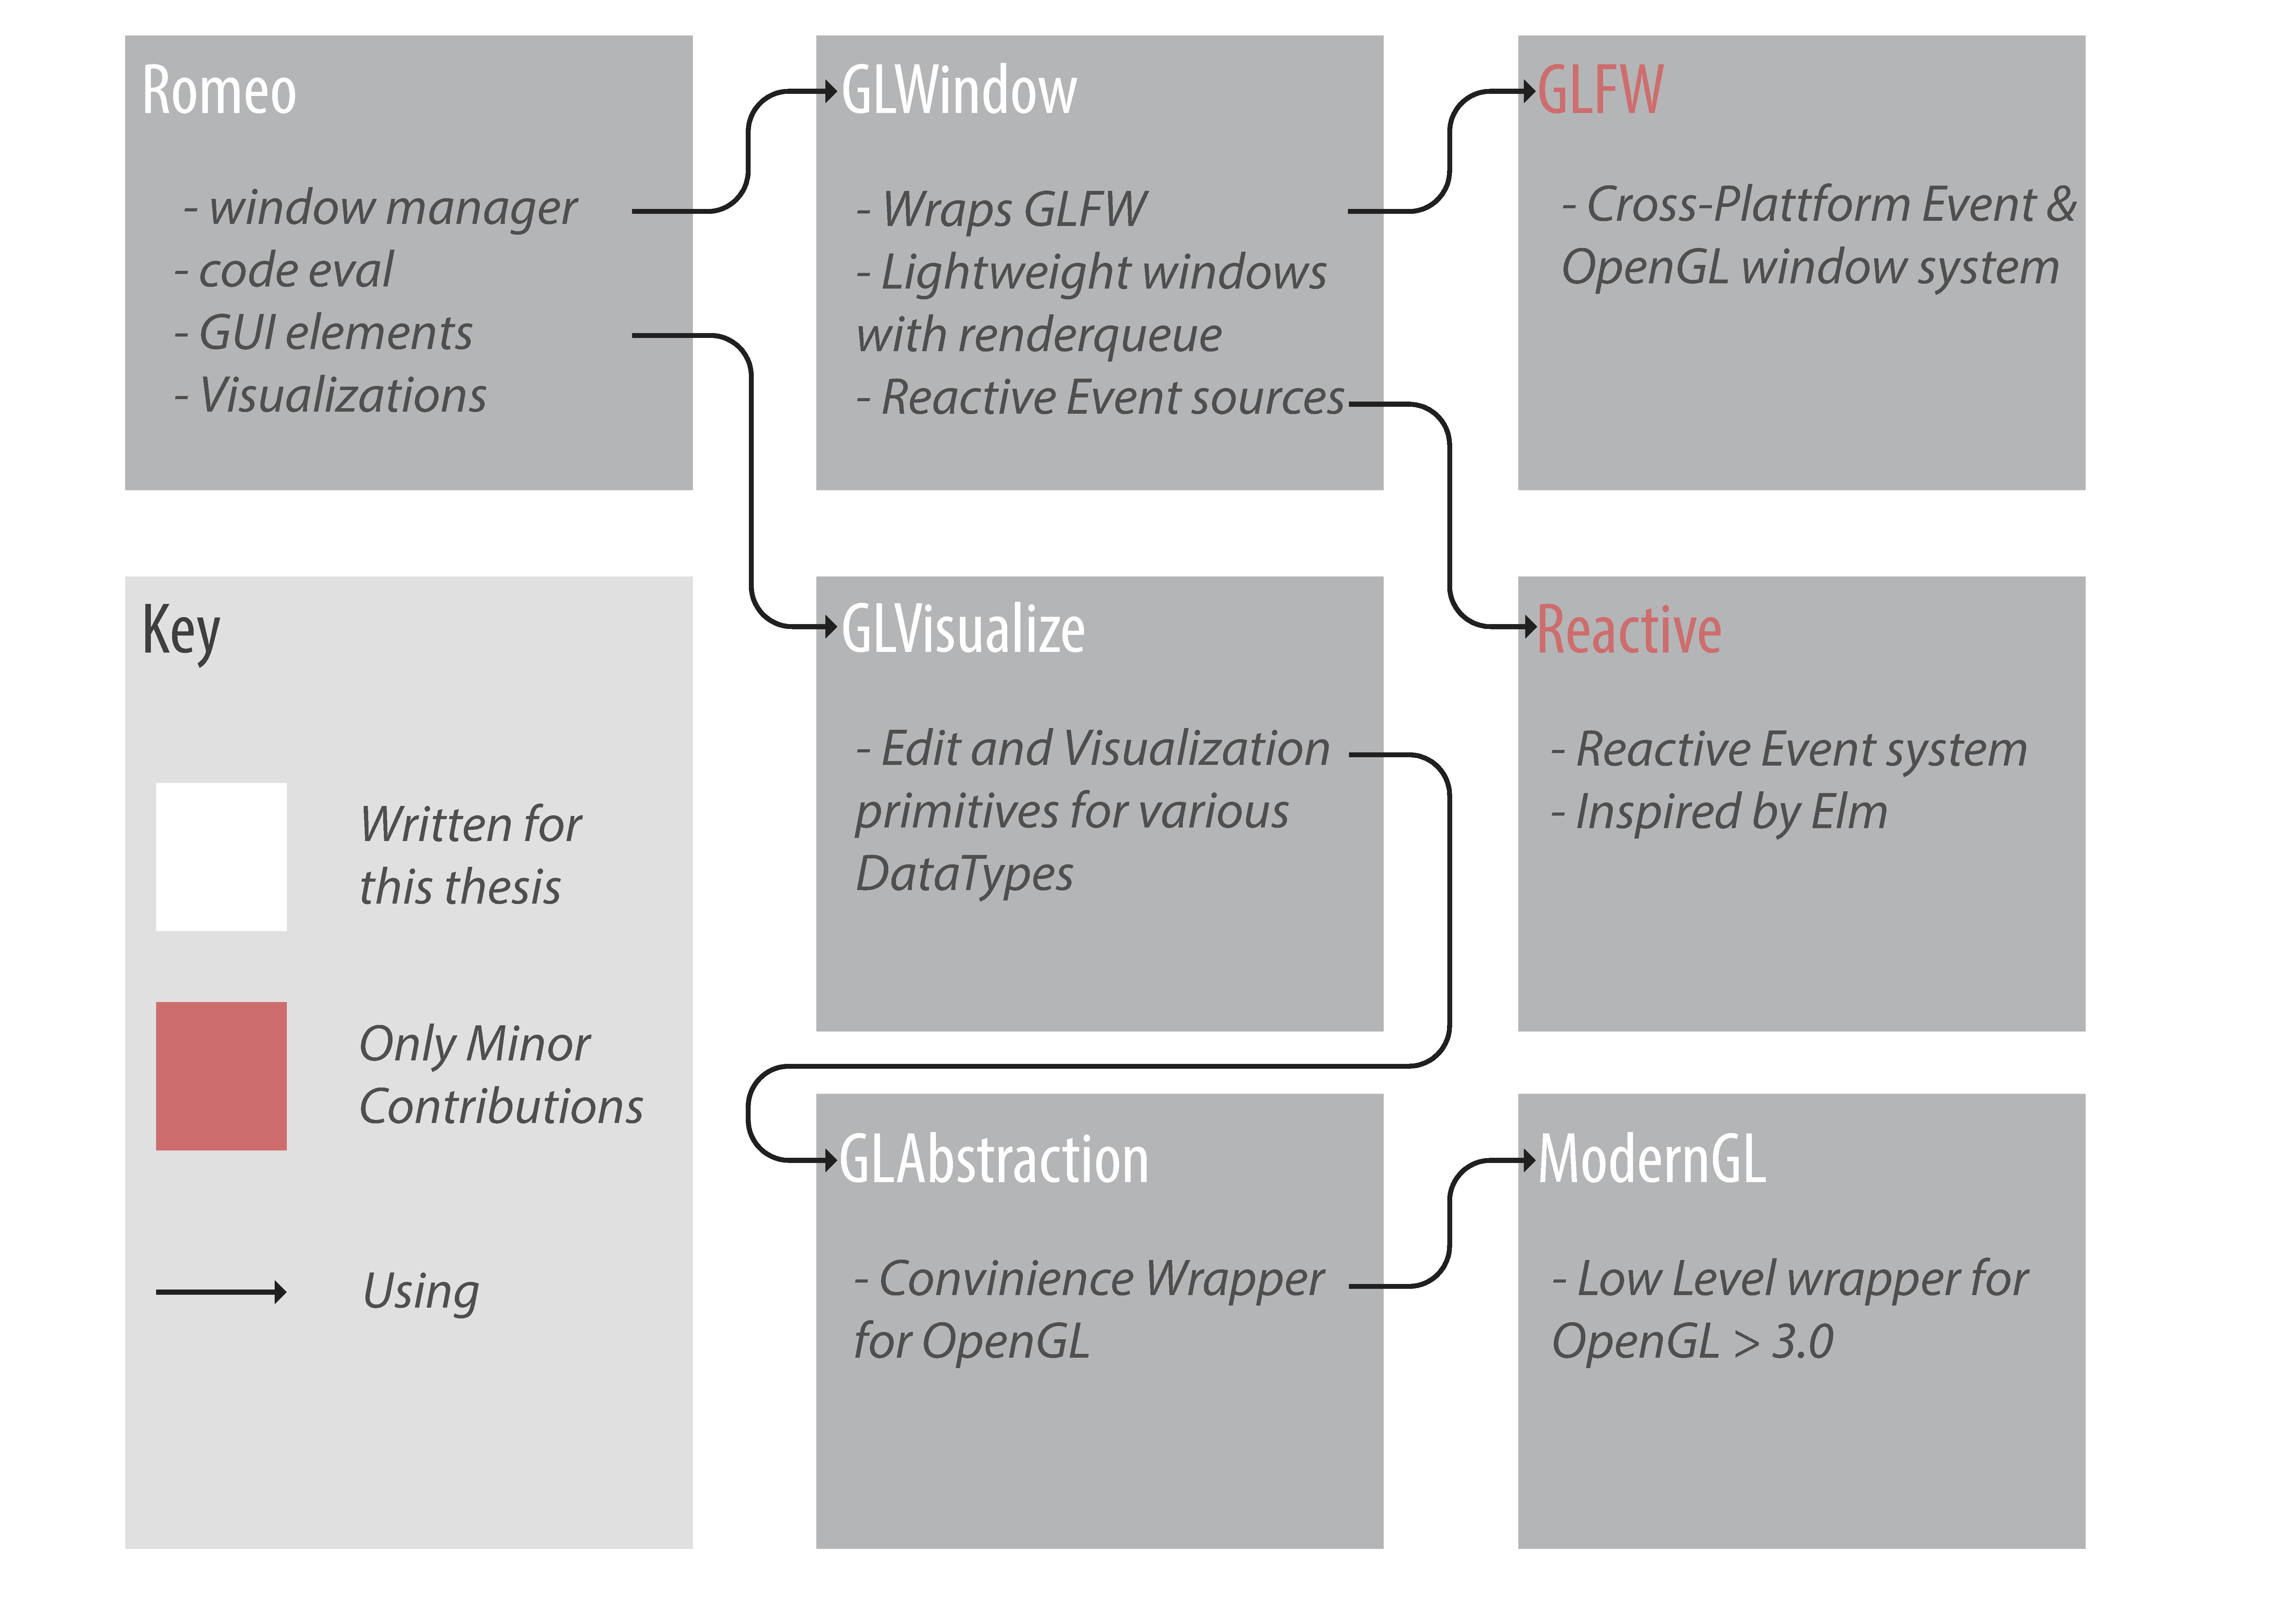
\includegraphics[width=0.9\linewidth]{graphics/architecture.pdf}
    \captionof{figure}[Architecture]{Main modules used in Romeo and their relation (simplified)}
    \label{fig:architecture} 
\end{minipage}
This chapter is about the architecture of Romeo.
Romeo itself just defines the high-level functionality of the editor.
This includes window layout and connecting all the different event sources to create the wanted behavior.
To do this, Romeo relies on a multitude of packages, which step for step abstract away the underlying low-level code that is used to do the window creation and rendering.
GLVisualize is the main package, offering the rendering functionality and the editor widgets, like text fields and sliders.
For rendering, GLVisualize relies on GLAbstraction, which defines a nice high-level interface to OpenGL.
OpenGL function loading is done by ModernGL, which keeps all the function and Enums definitions from OpenGL with version higher than 3.0.
The event management is handled by Reactive, which is a reactive event system written in Julia.

\subsection{Event System}
Holding everything together, since 1890.
\subsection{Low Level}

\subsubsection{ModernGL}
OpenGL is implemented by the video card vendor and is shipped via the video driver, which comes in the form of a C-Library.
The challenge is, to load the function pointer system and vendor independently. Also one further complication is, that depending on the platform, function pointer are only available after an OpenGL context was created and may only be valid for this context. \cite{wgl}
This problem is solved, by initializing a function pointer cache with null and as soon as the function is called the first time the real pointer gets loaded. This is suboptimal, as the pointer cannot be inlined and has to be checked for null.
In the newest version of Julia, this can be implemented even more efficiently with staged functions. Staged functions can be thought of as a runtime macro.
At the first call of the function, code can be generated, which then will get compiled in time and replaces the function definition. 
This makes the an OpenGL function call nearly twice as fast.
Like this, even C can be outperformed in terms of speed, as C doesn't have just in time compilation capabilities, so the function pointers can not be inlined like this.


\subsubsection{GLAbstraction}


\subsubsection{GLFW}
\subsubsection{GLWindow}

\subsection{High Level}

\subsubsection{GLVisualize}
\subsubsection{Romeo}
